\section{Task X}
\subsection{What you want to analyze}
We analyzing the rest of the data, we noticed that some machines had multiple
error types.  We estimated that these nodes had a larger problem, such as a
faulty motherboard.

\subsection{Why that is important}
If one is not careful and sees a series of memory errors, it is possible to keep
installing new memory when it is not the culprit.  Also, as motherboard
components tend to handle communication with I/O devices, there could be a
concern about silent data corruption or possible fault propagation. 

\subsection{What are your findings}
Fig. \ref{fig:taskx} contains a histogram that counts the nodes by 
the number of error types they exhibit in the sample dataset.  One can see that
while the number of machines with each error type decays exponentially, there
are still machines with three or more types of errors.  These machines likely
have a CPU/motherboard problem.  In Fig. \ref{fig:taskx_types}, we plot the
number of errors caused by machines against their number of error types.  Here,
it is clear that even though machines with 4 or 5 error types are the minority
in terms of nodes with errors, they represent a little less than half of all
errors generated.
\begin{figure}[h]
  \centering
  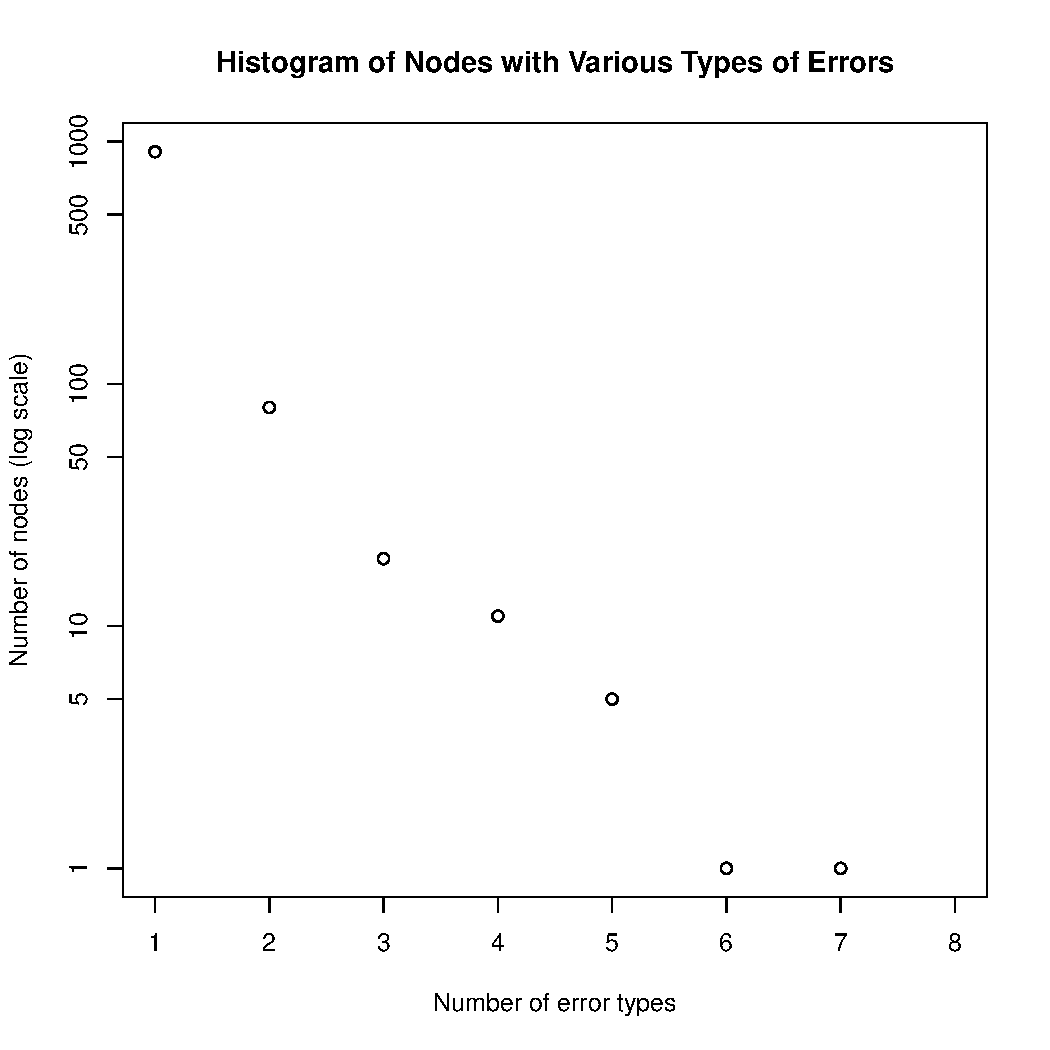
\includegraphics[width=0.45\textwidth]{images/taskx}
  \caption{Histogram of number of error types per nodes. The y axis is a log
  scale}\label{fig:taskx}
\end{figure}
\begin{figure}[h]
  \centering
  \includegraphics[width=0.45\textwidth]{images/taskx_types}
  \caption{Number of errors caused by nodes experiencing that many error types.
  }\label{fig:taskx_types}
\end{figure}
